\documentclass[../main.tex]{subfiles}
\begin{document}
\onlyinsubfile{
%\setcounter{chapter}{2}
}
\notinsubfile{}
\iffalse%---debug---
\fi%---debug---

\subsection*{Shor's algoritme en encryptie- eruit}

Vaak wil je een boodschap versturen die alleen voor de ontvanger bestemd is. Bijvoorbeeld als je een betaling wilt doen met je telefoon. Je kunt de boodschap dan versleutelen. De zender (Alice) bewerkt de boodschap met een recept dat alleen aan de ontvanger (Bob) bekend is. Het recept is de sleutel. Na versleuteling kan de boodschap gewoon over een publiek kanaal verzonden worden. De boodschap lijkt voor buitenstaanders onbegrijpelijk. Bob kan het recept omgekeerd toepassen (de inverse sleutel) en de boodschap leesbaar maken. 

Een eenvoudig voorbeeld: Versleutel de boodschap door alle letters in een boodschap een plaats verder in het alfabet te zetten. Dus A~$\rightarrow$~B, \ldots, L~$\rightarrow$~M,… Z~$\rightarrow$~A. Het omgekeerde recept is natuurlijk A~$\rightarrow$~Z,\ldots,L~$\rightarrow$~K,\ldots, Z~$\rightarrow$~Y. Nbllfjkl uf lsblfo.

Dit voorbeeld is wel heel \textit{makkelijk te kraken}. Het wordt interessanter als het ontcijferen een stuk moeilijker is dan het versleutelen. Met een sleutel moet de ontvanger natuurlijk wel makkelijk de boodschap kunnen ontcijferen. Een voorbeeld van zo'n asymmetrisch systeem is het volgende. Het is makkelijk twee grote priemgetallen te vermenigvuldigen tot een groot product. Het is heel moeilijk uit dit grote product de priemgetallen te achterhalen. Als je een van de factoren kent is het weer simpel. Met een deling vindt de ontvanger de factor terug. Hierop is het RSA systeem gebaseerd, het encryptiesysteem van onder andere onze banktransacties. Een klassieke computer kost het een eeuwigheid om moderne RSA te kraken. Peter Shor bedacht een quantumoplossing die de ontcijfering enorm kan versnellen. Als het systeem te kraken is heeft dit grote gevolgen. Gelukkig kan quantum ook daar weer een oplossing biden. Het gaat te ver om het RSA systeem helemaal te behandelen en ook het quantumalgoritme kunnen we niet helemaal behandelen (zie hiervoor bijvoorbeeld \cite{Veenstra2018}. Dit is echter zo'n belangrijke toepassing dat we een poging wagen.


\textbf{Getaltheorie} Om de priemgetallen te vinden zouden we het grote getal telkens kunnen testen met de vraag: is het deelbaar door 2,3,5,7,\ldots). Een klassieke computer moet de vragen een voor een beantwoorden, maar een quantumcomputer zou deze vragen in principe in een keer stellen omdat we gebruik kunnen maken van superpositie. Helaas, dat gaat hem niet worden. De vraag op die manier stellen is kansloos. Het goede antwoord zal homeopatisch verdeeld aan de uitgang verschijnen en we hebben een heel kleine kans dat we bij meting het goede antwoord treffen. Je kunt de quantumcomputer immers maar een keer uitlezen; het antwoord is een realisatie van een kansproces. Net zo goed als je met een enkel foton in onze experimenten in hofdstuk~\ref{chap:H1} waarschijnlijk niet kan achterhalen of je met een enkel of dubbelspleet te doen hebt. De strategie bij quantumcomputing is om de berekening zeer vaak uit te voeren, en een algoritme te schrijven waarbij constructieve en destructieve interferentie het juiste antwoord uit de kansverdeling boven laat drijven. 

De getaltheorie is een tak wan wiskunde die eigenschappen van getallen bestudeert. Methoden om de grootst gemene deler  te vinden waren al in de oudheid bekend. Een belangrijke eigenschap voor twee getallen (a, N). N is het product van de twee priemgetallen en voor a is met de methode van Euclides vastgesteld dat er geen gemeenschappelijke factoren zijn. Er geldt dat als je a voldoende keren met zichzelf vermenigvuldigt, dit je een veelvoud van N plus 1 oplevert. In formule:

$a^p=mN+1$, daarbi is $m$ een geheel getal.
We kunnen het omwerken om $m$ uit isoleren: $(a^p -1)/b=m$
Voorbeeld (a,N)=(7, 15) (a, N delen geen factoren)
\[\begin{aligned}
a^1:\quad &(7^1-1)/15=(7-1)/15=0.5 \quad mis\\
a^2:\quad &(7^2-1)/15=(49-1)/15=3.2 \quad mis\\
a^3:\quad &(7^3-1)/15=(343-1)/15=22.8 \quad mis\\
a^4:\quad &(7^4-1)/15=343-1/15=(2401-1)/15=160 \quad bingo!
\end{aligned}\]
Verzin zelf het eens (bijvoorbeeld N=9 a=5)

We schrijven het verband als  $a^p -1=mN$ en passen toe dat $(a-b)(a+b)=a^2-b^2$:
\[(ap/2-1)(ap/2+1) = mN\]
We hebben nu een vorm waarin twee ongelijke factoren staan die een veelvoud van $N $ opleveren. Dat komt in de richting: twee factoren de (een veelvoud) van $N$ beschrijven. We hebben het probleem nu ingewisseld voor een nieuw probleem: het vinden van de periodiciteit van $p$. De herhaling in ons rekenvoorbeeld heeft een periode 4. 

Stel je bent proefpersoon in een experiment waarin je eigen bioritme wordt bepaald. In het experiment verblijf je in een kamer zonder ramen, en zonder contact met de buitenwereld. Je wordt je uit jezelf wakker en je gaat uit jezelf naar bed als je moe bent. In de kamer hangen een aantal 24-uurs klokken met alleen een uurwijzer. Onder de klokken hangt een papiertje waarop je een streepje met een centimeter verlengt in de richting van de wijzer als je wakker wordt. De klokken lopen allemaal in een verschillend tempo, te snel of te langzaam. Als de klok veel te snel of veel te langzaam loopt, komen na een paar dagen de streepjes in willekeurige richting te staan en blijven ze op het papiertje. Maar op het papiertje onder de klok die gelijk loopt met jouw bioritme komt het streepje telkens in dezelfde richting te staan. Je bent al gauw van het papier af. Op deze manier kun je destructieve en constructieve interferentie een oplossing boven. Een proces dat je resonantie kunt noemen.
De klokken in het voorbeeld zijn in een quantumcomputer qubits die ronddraaien op de eenheidscirkel.. Ze zijn geprogrammeerd om ieder hun eigen frequentie te draaien. 
Er is een wiskundige operatie Fouriertransformatie, waarmee je een signaal zonder informatieverlies uit kunt drukken in zijn omgekeerde. Meestal van tijd naar frequentie of van afstand naar dichtheid (1/afstand). Zo zijn de patronen op de muur en in het kaartje bij ons spletenexperiment elkaars Fourier-getransformeerde. De transformatie kan zowel heen als terug zonder verlies van informatie, wat natuurlijk een voorwaarde is voor een quantumversie vaan de Fouriertransformatie (waarom?).
Een Fouriertransformatie kan een signaal analyseren en in een keer het goede antwoord oven laten drijven.

Het was de geniale stap van Peter Shor om het verband tussen deze technieken te zien en zo een althans in theorie het RSA systeem te kraken. Het wachten is op de hardware.

Nu is encryptie een wapenwedloop tussen versleutelaars en krakers. Met RSA stonden de versleutelaars heel lang voor. De gevolgen van Shor's algoritme zijn groot. Informatie die (sinds decennia) versleuteld on-line is komen te staan zal dan een open boek izjn. Gelukkig is de volgende stap in de wapenweddloop weer gezet. Post quantumencryptie. Een eenvoudig voorbeeld van quantumversleuteling vind je in opdracht \nogdoen{BB84}.

\newcommand\klok[2][2]{%
\begin{tikzpicture}[scale=#1,line cap=round,line width=#1*3pt]
\filldraw [fill=yellow!20] (0,0) circle (2cm);
\foreach \angle / \label in
{0/6, 30/4, 60/2, 90/24, 120/22, 150/20, 180/18,
210/16, 240/14, 270/12, 300/10, 330/8}
{
\draw[line width=#1*1pt] (\angle:1.8cm) -- (\angle:2cm);
\draw (\angle:1.4cm) node[scale=#1]{\textsf{\label}};
}
\foreach \angle in {0,90,180,270}
\draw[line width=#1*2pt] (\angle:1.6cm) -- (\angle:2cm);
\node[draw=none,font=\tiny,text=red,scale=#1] at (0,.9cm) {Quantim};
\draw[rotate=90,line width=#1*2pt] (0,0) -- (-#2*15:0.7cm); % hours
\path [fill=black] (0,0) circle (3pt);
\path [fill=red] (0,0) circle (1.5pt);
%
\end{tikzpicture}%
}
%%\syntax
%% \clock[<optional scaling dim>]{<hour>}

\noindent\klok[.4]{6}\quad\klok[.4]{7}\quad\klok[.4]{8}\quad\klok[.4]{9}\quad\klok[.4]{10}
  

\begin{flushleft}
\begin{minipage}{.45\textwidth}
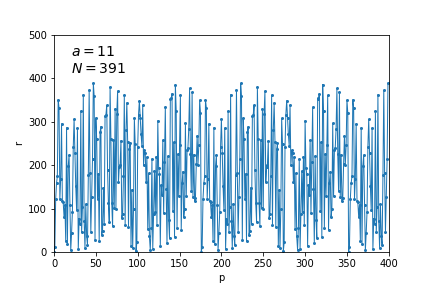
\includegraphics[width=\textwidth]{./img/shorN=391a=11.png}
\end{minipage}%
\hfill
\begin{minipage}{.5\textwidth}
 \captionof{figure}{repeterende rest. De functie$ r=a^p mod N$ ziet er grillig uit. Kun je de herhalingsperiode vinden? \label {fig:shorrest}}
\end{minipage}%
\end{flushleft}

\end{document}